\addcontentsline{toc}{chapter}{Занятие 14. Цепи Маркова. Классификация состояний.}
\chapter*{Занятие 14. Цепи Маркова. Классификация состояний.}

\addcontentsline{toc}{section}{Контрольные вопросы и задания}
\section*{Контрольные вопросы и задания}

\subsubsection*{Приведите определение цепи Маркова.}

Последовательность дискретных случайных величин $ \left\{ x_n \right\}_{n \geq 0}$
называется простой цепью Маркова (с дискретным временем), если
\begin{equation*}
  P \left( x_{n + 1} = i_{n + 1} \; \middle| \; x_n = i_n, \dotsc, x_0 = i_0 \right) =
  P \left( x_{n + 1} = i_{n + 1} \; \middle| \; x_n = i_n \right).
\end{equation*}

\subsubsection*{Что называется переходными вероятностями цепи Маркова?}

Матрица $P \left( n \right) $,
где $P_{ij} \left( n \right) = P \left( x_{n + 1} = i_{n + 1} \; \middle| \; x_n = i \right) $,
называется матрицей переходных вероятностей на $n$-м шаге.

\subsubsection*{Как вычисляются переходные вероятности цепи Маркова за $n$ шагов?}

Матрица переходных вероятностей за $n$ шагов однородной цепи Маркова есть $n$-я
степень матрицы переходных вероятностей за 1 шаг.

\subsubsection*{Запишите уравнение Колмогорова-Чепмена.}

$P \left( x_n - i_n \; \middle| \; x_0 = i_0 \right) =
  \left( P^n \right)_{i_0, i_n}$.

\subsubsection*{Опишите, как классифицируются состояния цепи Маркова.}

Группы состояний марковской цепи (подмножества вершин графа переходов),
которым соответствуют тупиковые вершины диаграммы порядка графа переходов,
называются эргодическими классами цепи.
Состояния, которые находятся в эргодических классах, называются существенными,
а остальные~---~несущественными.
Поглощающее состояние является частным случаем эргодического класса.
Тогда попав в такое состояние, процесс прекратится.

\addcontentsline{toc}{section}{Аудиторные задачи}
\section*{Аудиторные задачи}

\subsubsection*{14.2}

\textit{Задание.}
Подбрасывается игральный кубик.
Выясните
образует ли последовательность $ \left\{ \xi_n \right\}_{n \geq 1}$ однородную цепь Маркова, если
\begin{enumerate}[label=\alph*)]
  \item $ \xi_n$~---~это наибольшее из чисел, которые выпали в первых $n$ подбрасываниях;
  \item $ \xi_n$~---~это количество шестёрок, которые выпали в первых $n$ подбрасываниях.
\end{enumerate}

\textit{Решение.}
\begin{enumerate}[label=\alph*)]
  \item $ \xi_n = \max \left( x_1, \dotsc, x_n \right) $,
  где $x_1, x_2, \dotsc, x_n$~---~это результаты подбрасываний кубика
  (принимают значения $1, \dotsc, 6$).
  Нужно проверить, что вероятность зависит только от $j$ и $i_n$.
  Попробуем $ \xi_{n + 1}$ переписать через $ \xi_n$.
  Напишем рекуррентное соотношение $ \xi_{n + 1} = \max \left( \xi_n, x_{n + 1} \right) $.
  Подставим это в формулу
  \begin{gather*}
    P \left( \xi_{n + 1} = j \; \middle| \; \xi_1 = i_1, \dotsc, \xi_n = i_n \right) = \\
    = P \left\{
      \max \left( \xi_n, x_{n + 1} \right) = j \; \middle| \; \xi_1 = i_1, \dotsc, \xi_n = i_n
    \right\} =
  \end{gather*}
  Знаем, что $ \xi_n = i_n$.
  Тогда
  \begin{equation*}
    = P \left\{
      \max \left( i_n, x_{n + 1} \right) = j \; \middle| \; \xi_1 = i_1, \dotsc, \xi_n = i_n
    \right\} =
  \end{equation*}
  Случайная величина $ \max \left( i_n, x_{n + 1} \right) $ зависит только от $x_{n + 1}$.
  Условие зависит только от $x_1, \dotsc, x_n$.
  Событие и условие независимы.
  Эта вероятность станосится безусловной
  \begin{equation*}
    = P \left\{ \max \left( i_n, x_{n + 1} \right) = j \right\} =
  \end{equation*}
  Вывод: вероятность зависит только от $i_n$ и $j$, так что это марковская цепь.
  Посчитаем вероятность
  \begin{equation*}
    = \begin{cases}
      0, \qquad i_n > j, \\
      P \left( x_1 \leq j \right), \qquad i_n = j, \\
      P \left( x_1 = j \right), \qquad i_n < j
  \end{cases} =
  \end{equation*}
  Случайная величина $x_1$ принимает значения с вероятностями $6^{-1}$.
  Таким образом, получаем
  \begin{equation*}
    = \begin{cases}
        0, \qquad i_n > j, \\
        \frac{j}{6}, \qquad i_n = j, \\
        \frac{1}{6}, \qquad i_n < j.
      \end{cases}
  \end{equation*}

  Значит, можно теперь нарисовать матрицу переходных вероятностей
  \begin{equation*}
    \bordermatrix{i_n \ j & 1 & 2 & 3 & 4 & 5 & 6 \cr
                  1 & \frac{1}{6} & \frac{1}{6} & \frac{1}{6} & \frac{1}{6} & \frac{1}{6} & \frac{1}{6}\cr
                  2 & 0 & \frac{2}{6} & \frac{1}{6} & \frac{1}{6} & \frac{1}{6} & \frac{1}{6} \cr
                  3 & 0 & 0 & \frac{3}{6} & \frac{1}{6} & \frac{1}{6} & \frac{1}{6} \cr
                  4 & 0 & 0 & 0 & \frac{4}{6} & \frac{1}{6} & \frac{1}{6} \cr
                  5 & 0 & 0 & 0 & 0 & \frac{5}{6} & \frac{1}{6} \cr
                  6 & 0 & 0 & 0 & 0 & 0 & 1 \cr}
  \end{equation*}

  Получилая верхнедиагональная матрица.
  В каждой строчке сумма~---~единица.
  \item Нужно начинать с того, что написать формулу для $ \xi_n$, чтобы представить его через $x$.

  \begin{equation*}
    \xi_n =
    \sum \limits_{i = 1}^n \mathbbm{1} \left\{ x_i = 6 \right\} =
  \end{equation*}
  Видели, что удобно иметь рекурентное соотношение
  \begin{equation*}
    = \sum \limits_{i = 1}^{n - 1} \mathbbm{1} \left\{ x_i = 6 \right\} +
    \mathbbm{1} \left\{ x_n = 6 \right\} =
    \xi_{n - 1} + \mathbbm{1} \left\{ \xi_n = 6 \right\}.
  \end{equation*}
  Проверим, что это марковская цепь.

  Подставим в вероятность выражение для $ \xi_n$ через $ \xi_{n - 1}$, то есть
  \begin{gather*}
    P \left( \xi_n = j \; \middle| \; \xi_{n - 1} = i_{n - 1}, \dotsc, \xi_1 = i_1 \right) = \\
    = P \left(
      \xi_{n - 1} + \mathbbm{1} \left\{ x_n = 6 \right\} = j \; \middle| \;
      \xi_{n - 1} = i_{n - 1}, \dotsc, \xi_1 = i_1
    \right) = \\
    = P \left(
      i_{n - 1} + \mathbbm{1} \left\{ x_n = 6 \right\} = j  \; \middle| \;
      \xi_{n - 1} = i_{n - 1}, \dotsc, \xi_1 = i_1
    \right) =
  \end{gather*}
  Событие и условие независимы, опять вероятность безусловная
  \begin{equation*}
    = P \left( i_{n - 1} + \mathbbm{1} \left\{ x_n = 6 \right\} = j \right) =
  \end{equation*}
  Из этого уже следует, что это марковская цепь
  \begin{equation*}
    = P \left( \mathbbm{1} \left\{ x_1 = 6 \right\} = j - i_{n - 1} \right) =
    \begin{cases}
      \frac{1}{6}, \qquad j = i_{n - 1} + 1, \\
      \frac{5}{6}, \qquad j = i_{n - 1}, \\
      0, \qquad in \, all \, other \, cases.
    \end{cases}
  \end{equation*}

  У нас получилась марковская цепь с такими переходными вероятностями
  \begin{equation*}
    \bordermatrix{~ & 0 & 1 & 2 & 3 & \dotsc \cr
                  0 & \frac{5}{6} & \frac{1}{6} & 0 & 0 & \dotsc \cr
                  1 & 0 & \frac{5}{6} & \frac{1}{6} & 0 & \dotsc \cr
                  2 & 0 & 0 & \frac{5}{6} & \frac{1}{6} & \dotsc \cr
                  3 & 0 & 0 & 0 & \frac{5}{6} & \dotsc \cr
                  \dotsc & \dotsc & \dotsc & \dotsc & \dotsc & \dotsc \cr}
  \end{equation*}

  Сейчас матрица бесконечна.
\end{enumerate}

\subsubsection*{14.5}

\textit{Задание.}
Пусть $ \left\{ X_n, \, n \geq 0 \right\} $~---~однородная цепь Маркова с множеством состояний
$E = \left\{ 1, 2, 3 \right\} $, матрицей переходных вероятностей
\begin{equation*}
  P =
  \begin{bmatrix}
    0 & \frac{1}{3} & \frac{2}{3} \\
    \frac{1}{4} & \frac{3}{4} & 0 \\
    \frac{2}{5} & 0 & \frac{3}{5}
  \end{bmatrix}
\end{equation*}
и начальным распределением
\begin{equation*}
  p_0 =
  \left( \frac{2}{5}, \frac{1}{5}, \frac{2}{5} \right).
\end{equation*}
Вычислите:
\begin{enumerate}[label=\alph*)]
  \item $P \left( X_1 = 2, X_2 = 2, X_3 = 2, X_4 = 1, X_5 = 3 \right) $;
  \item $P \left( X_5 = 2, X_6 = 2 \; \middle| \; X_2 = 2 \right) $;
  \item $P \left( X_2 = 3 \right) $.
\end{enumerate}

\textit{Решение.}
У такой цепи есть 3 состояния и переходы (рис. \ref{fig:145}).

\begin{figure}[h!]
  \centering
  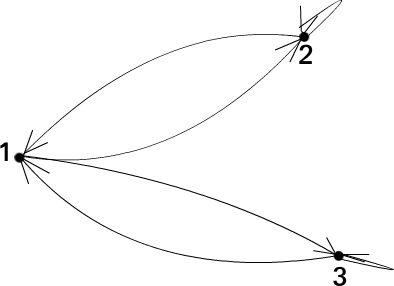
\includegraphics[width=.4\textwidth]{./pictures/14_5.png}
  \caption{Состояния и переходы цепи Маркова}
  \label{fig:145}
\end{figure}

Посчитаем вероятность того, что
\begin{enumerate}[label=\alph*)]
  \item \begin{gather*}
    P \left( X_1 = 2, X_2 = 2, X_3 = 2, X_4 = 1, X_5 = 3 \right) = \\
    = \frac{2}{5} \cdot \frac{1}{3} \cdot \frac{3}{4} \cdot \frac{3}{4} \cdot \frac{1}{4} \cdot
    \frac{2}{3} +
    \frac{1}{5} \cdot \frac{3}{4} \cdot \frac{3}{4} \cdot \frac{1}{4} \cdot \frac{2}{3} +
    \frac{2}{5} \cdot 0;
  \end{gather*}
  \item \begin{equation*}
    P \left( X_5 = 2, X_6 = 2 \; \middle| \; X_2 = 2 \right) =
    P \left( 2 \to \to \to 2 \to 2 \right) =
  \end{equation*}
  Надо перебрать все возможные варианты
  \begin{gather*}
    = P \left( 2 \to 2 \to 2 \to 2 \to 2 \right) + P \left( 2 \to 2 \to 1 \to 2 \to 2 \right) + \\
    + P \left( 2 \to 1 \to 2 \to 2 \to 2 \right).
  \end{gather*}
  Для каждого слагаемого нужно поперемножать вероятности.
\end{enumerate}

\subsubsection*{14.6}

\textit{Задание.}
По виду матрицы переходных вероятностей проведите классификацию состояний соответствующей цепи
Маркова
\begin{equation*}
  P =
  \begin{bmatrix}
    \frac{1}{2} & 0 & \frac{1}{2} & 0 & 0 \\
    0 & \frac{1}{2} & 0 & 0 & \frac{1}{2} \\
    0 & 0 & 0 & 1 & 0 \\
    \frac{1}{3} & 0 & \frac{1}{3} & \frac{1}{3} & 0 \\
    \frac{1}{2} & 0 & 0 & 0 & \frac{1}{2}
  \end{bmatrix}.
\end{equation*}

\textit{Решение.}
$i \leftrightarrow j$~---~сообщающиеся, если есть путь из $i$ в $j$, и есть путь из $j$ в $i$.

Если существует $j$ такой, что $i \to j, \, j \not \to i$, то $i$~---~несущественное.

Если существует путь из $i$ в $j$, то $j$~---~достижимое.

\begin{figure}[h!]
  \centering
  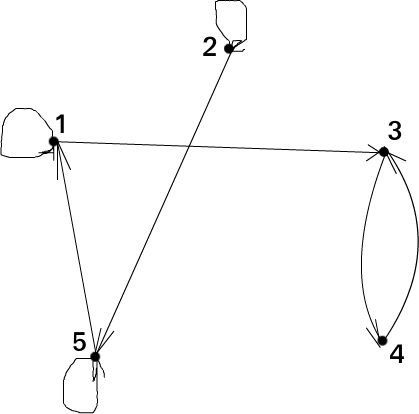
\includegraphics[width=.4\textwidth]{./pictures/14_6.png}
  \caption{Состояния и переходы цепи Маркова}
  \label{fig:146}
\end{figure}

Сообщающиеся: $3 \leftrightarrow 4, \, 1 \leftrightarrow 3$ (рис. \ref{fig:146}).

Несущественные: $2, 5$.

Существенные: $ \left\{ 1, 3, 4 \right\} $, несущественные:
$ \left\{ 2 \right\}, \, \left\{ 5 \right\} $.

\addcontentsline{toc}{section}{Домашнее задание}
\section*{Домашнее задание}

\subsubsection*{14.10}

\textit{Задание.}
Пусть $ \left\{ Y_i \right\}_{i \geq 1}$
является последовательностью независимых одинаково распределённых дискретных случайных величин,
\begin{equation*}
  P \left( Y_1 = k \right) = p_k, \,
  k = 0, 1, 2, \dotsc.
\end{equation*}
Положим $X_0 = 0, \, X_n = Y_1 + \dotsc + Y_n, \, n \geq 1$.
Докажите, что последовательность $ \left\{ X_n \right\}_{n \geq 0}$ образует цепь Маркова.
Найдите его переходные вероятностии начальное распределение.

\textit{Решение.}
Убедимся, что последовательность $ \left\{ X_n \right\}_{n \geq 0}$ образует цепь Маркова.
Действительно,
для произвольного $n \geq 1$ и произвольных целых чисел $i_0, i_1, \dotsc, i_n \geq 0$ имеем:
\begin{equation*}
  P \left( X_0 = i_0, X_1 = i_1, \dotsc, X_n = i_n \right) =
\end{equation*}
Выразим через случайные величины $Y_i$ и получим
\begin{equation*}
  = P \left( X_0 = i_0, Y_1 = i_1 - i_0, \dotsc, Y_n = i_n - i_{n - 1} \right) =
\end{equation*}
Все события независимы
\begin{gather*}
  = P \left( X_0 = i_0 \right) \cdot P \left( Y_1 = i_1 - i_0 \right) \cdot \dotsc \cdot
  P \left( Y_n = i_n - i_{n - 1} \right) = \\
  = \begin{cases}
    p_{i_1 - i_0} \cdot \dotsc \cdot p_{i_n - i_{n - 1}}, \qquad
    i_0 = 0, \, i_1 - i_0, \dotsc, i_n - i_{n - 1} \in \mathbb{N} \cup \left\{ 0 \right\}, \\
    0, \qquad otherwise.
  \end{cases}
\end{gather*}

Таким образом,
\begin{gather*}
  P \left( X_0 = i_0, X_1 = i_1, \dotsc, X_{n + 1} = i_{n + 1} \right) = \\
  = P \left( X_0 = i _0, X_1 = i_1, \dotsc, X_n = i_n \right) \cdot p_{i_n i_{n + 1}},
\end{gather*}
где
\begin{equation*}
  p_{ij} =
  P \left( X_{n + 1} = j \; \middle| \; X_n = i \right) =
  \begin{cases}
    p_{j - i}, \qquad j - i \in \mathbb{N} \cup \left\{ 0 \right\}, \\
    0, \qquad otherwise,
  \end{cases}, \, i \in \mathbb{Z}, \, i \geq 0.
\end{equation*}

Значит, $ \left\{ X_n, \, n \geq 0 \right\} $
образует цепь Маркова с матрицей переходных вероятностей
\begin{equation*}
  P =
  \begin{bmatrix}
    p_0 & p_1 & p_2 & p_3 & \dotsc \\
    0 & p_0 & p_1 & p_2 & \dotsc \\
    0 & 0 & p_0 & p_1 & \dotsc \\
    \dotsc & \dotsc & \dotsc & \dotsc & \dotsc
  \end{bmatrix}
\end{equation*}

Начальное распределение $p_0 = \left( 1, 0, 0, 0, \dotsc \right) $.

\subsubsection*{14.12}

\textit{Задание.}
Пусть $ \left\{ \xi_n, \, n \geq 0 \right\} $~---~простое случайное блуждание на $ \mathbb{Z}$,
то есть цепь Маркова с переходными вероятностями $p_{i, i + 1} = p, \, p_{i, i - 1} = 1 - p$.
Найдите вероятности перехода за $n$ шагов.

\textit{Решение.}
Есть случайное блуждание с вероятностями
\begin{equation*}
  P \left( \xi_{n + 1} = \xi_n + 1 \right) = p, \,
  P \left( \xi_{n = 1} = \xi_n - 1 \right) = 1 - p.
\end{equation*}

Имеем переходные верояности
\begin{equation*}
  p_{ij} =
  \begin{cases}
    p, \qquad j = i + 1, \\
    1 - p, \qquad j = i - 1, \\
    0, \qquad otherwise.
  \end{cases}
\end{equation*}

За 2 шага переходные вероятности равны
\begin{equation*}
  p_{ij}^{ \left( 2 \right) } =
  \begin{cases}
    p^2, \qquad j = i + 2, \\
    \left( 1 - p \right)^2, \qquad j = i - 2, \\
    2p \left( 1 - p \right), \qquad i = j, \\
    0, \qquad otherwise.
  \end{cases}
\end{equation*}

Нужно найти переходные вероятности за $n$ шагов
\begin{gather*}
  P \left( \xi_n = k \right) =
  P \left(
    there \, are \, k + \frac{n - k}{2} steps \, up, \frac{n - k}{2} steps \, down
  \right) = \\
  = C_n^{ \frac{n - k}{2}} \left( 1 - p \right)^{ \frac{n - k}{2}} p^{k + \frac{n - k}{2}}.
\end{gather*}
